\documentclass[conference]{IEEEtran}

\usepackage[pdftex]{graphicx}
\usepackage[cmex10]{amsmath}
\usepackage{algorithmic}
\usepackage{caption}
\usepackage{subfig}
\usepackage{url}
\usepackage{balance}

\begin{document}
%\title{ What GitHub and Google Code can tell us about the Causes of Crashes of Android Apps? }
%\title{ A Mining Study the Google Code can tell us about the Causes of Crashes of Android Apps? }

%\title{What can the Issues of GitHub and Google Code tell us about Exception Fragilities? }

\title{What can Issues on GitHub and Google Code tell us about Bug Hazards in Android and Java? }

%\title{Results of a Mining Study on Exception Stack Traces embedded on issues of over 600 Android Projects}

%\title{Unveiling Robustness Threats by Mining the Exception Stack Traces of over 600 Android Projects}

%\title{Discovering Threats to Robustness through Exception Stack Trace Analysis: Results of a Mining Study of Android Projects}

%\title{Discovering Threats to Robustness through Exception Stack Trace Mining}

%\title{Discovering Threats to Robustness through Exception Stack Trace Mining of over 600 Android Projects}

%\title{Discovering Threats to Robustness through a Mining Study of Exception Stack Traces}

%\title{Discovering Fragilities on the Exception-Related Code through  Exception Stack Trace Mining}

%\title{On the Common Characteristics Android-Apps Crashes: Results of a GitHub and Google Code Mining Study}

%\title{On the Common Characteristics of Android-Apps Crashes: Results of a GitHub and Google Code Mining Study}

%\title{On the Common Characteristics of Android Crashes: Results of a GitHub and Google Code Mining Study}


%\title{A first Glance on Characteristics of Android Crashes: Results of a GitHub and Google Code Mining Study}


%\title{A first Glance on Characteristics of Android Crashes: Results of a GitHub and Google Code Mining Study}


\author{\IEEEauthorblockN{Roberta Coelho\IEEEauthorrefmark{1},
Lucas Almeida\IEEEauthorrefmark{1},
Georgios Gousios\IEEEauthorrefmark{2},
Arie van Deursen\IEEEauthorrefmark{3}
}
\IEEEauthorblockA{\IEEEauthorrefmark{1}Federal University of Rio Grande do Norte\\
Natal, Brazil\\
Email: \texttt{roberta@dimap.ufrn.br,lucas.almeida@ppgsc.ufrn.br}}
\IEEEauthorblockA{\IEEEauthorrefmark{2}Radboud University Nijmegen\\
Nijmegen, The Netherlands\\
Email: \texttt{georgios@cs.ru.nl}}
\IEEEauthorblockA{\IEEEauthorrefmark{3}Delft University of Technology\\
Delft, The Netherlands\\
Email: \texttt{arie.vandeursen@tudelft.nl}}
}

\newcommand{\todo}[1]{\textbf{TODO}\footnote{\textbf{TODO:} #1}}

% make the title area
\maketitle

%GitHub 31,592
% Google Code: 127,456
%All: 159,048
% bf: 31,592 (with exception)



%The goal of this study was to: identify common characteristics 
%of such traces and investigate the fragilities on the exception-related code that can be revealed
%from them. 
%The goal of this study was to: identify common characteristics 
%of such traces and investigate the whether they can reveal
%the characteristics on the source code that may be favoring the introduction of faults 
%(i.e. Uncaught Exceptions, and Unintened handler Actions), and consequently
%decreasing the program robustness.
%(of apps or the underlaying framework) 



\begin{abstract}
%The number of mobile apps is increasing in a daily rate. If on the one hand they
%extend phones capabilities far beyond of the basic calls, on the other hand they have to 
%cope with an increasing number of exceptional conditions 
%(e.g., faults in underlying middleware or hardware; memory and battery restrictions). 
%Therefore, mechanisms for exception detection and handling are not an optional add-on but a 
%fundamental part of such apps. However, studies have shown that such mechanisms are the less 
%understood and tested parts of the system. As a consequence they may affect the system the 
%other way around, making the system even less robust, leading to failures such as uncaught exceptions 
%and unintended handling (i.e., exceptions being mistakenly caught by existing handlers).

This paper reports on a study mining the exception stack traces included in
159,048 issues reported on Android projects hosted in GitHub (482 projects) 
and Google Code (157 projects). The goal of this study is to investigate 
whether stack trace information can reveal \emph{bug hazards} related to exception handling code that may lead to a decrease in application robustness. 
 Overall 6,005 exception stack traces were extracted, and subjected to source code and bytecode analysis. 
The outcomes of this study include the identification of the following 
\emph{bug hazards}: (i) unexpected cross-type exception wrappings (for instance, trying to handle an instance 
of OutOfMemoryError ``hidden'' in  a checked exception)  which can make the exception-related code 
more complex and negatively impact the application robustness; (ii) undocumented runtime exceptions 
thrown by both the Android platform and third party libraries; and (iii) undocumented checked exceptions
 thrown by the Android Platform. Such undocumented exceptions make difficult, and most of the times infeasible
for the client code to protect against ``unforeseen'' situations that may happen while calling third-party code.
This study provides further insights on such \emph{bug hazards} and the robustness threats  
they impose to Android apps as well as to other systems based on the Java exception model.

%A bug hazard is a circumstance that increases the chance of a bug to be present in the software.
\end{abstract}

%GitHub 31,592
% Google Code: 127,456
%All: 159,048


%Total page numbers then:
%intro:       1
%background:  1.5
%method:      1
%tool         0.5
%findings     4
%discussion   1
%threats      .5
%conc         .5
%------------------+
%total        10 pages


%\IEEEpeerreviewmaketitle

%Such increase is motivated by pervasiveness of the World Wide Web 
%and the unprecedented increase of global smartphone shipments -
%the mobile industry shipped over 315 million smartphones in the last quarter of 2013 ~\cite{googleio}.

%In this context, Android has become a leading platform - thanks to its open-source 
%model and hardware partners like Samsung, HTC, Motorola, Asus (besides Nexus Google's
% own device) ~\cite{gartner}.  Google estimates that there is over 1 billion Android active users per month ~\cite{googleio},
%and the number of apps built on top of Android increases in a daily rate.

%Our conjecture is that several Android applications may be suffering from common 
%fragilities on the exception-related code (of the applications themselves or 
%the underlaying platform) which may be degratind their robustness.
%We call ``fragilities" characteristics on the exception-related code that favor the introduction
%of aforementioned failures.

%In Java, when an application fails due to an uncaught exception, 
%it automatically terminates, while the system prints a stack trace to the console, 
%or log file ~\cite{gosling2000java}.  A typical Java stack trace consists of  the fully qualified name 
%the thrown exception and the ordered list of methods that were active on the call stack before 
%such exception has occurred ~\cite{gosling2000java,bloch2008effective}.
%and unintended handling~\cite{miller1997issues} (i.e., exceptions being mistakenly caught by existing handlers) 

\section{Introduction}

In recent years, we have witnessed an astonishing increase in the number of
mobile applications. These applications extend phones capabilities 
far beyond basic calls and textual messages. Such applications, however,
have to face an increasing number of threats to application robustness
 arising from failures in the underlying middleware and hardware (e.g., camera, sensors);
failures in third party services and libraries; compatibility issues~\cite{McDon13}; 
 memory and battery restrictions; and noisy external resources ~\cite{Zhang12} 
(e.g., wireless connections,GPS, bluetooth). 

Therefore, techniques for error detection and handling are not  an optional add-on but a 
fundamental part of such apps. The exception handling mechanism~\cite{goodenough1975exception},
embedded in many mainstream programming languages, such as Java, C++ and C\#,
 is one of the most used techniques for detecting and recovering from such exceptional conditions.
In this paper we will be concerned with exception handling in Android apps,
which reuses Java's exception handling model.
 
%Android, the leading plaform for mobile applications~\cite{gartner} (thanks to its open-source 
%model and hardware partners like Samsung, HTC, Motorola, Asus besides Nexus Google's
% own device)  reuses the embedded Java exception model to detect and handle 
% exceptional conditions.

Studies have shown that exception-related code is generally poorly understood and among the least tested parts of the system~\cite{miller1997issues,Robil00,shah2010understanding, 
garcia2007extracting,garcia2001comparative,cabral2007exception,coelho2011unveiling,yuan:2014.osdi}.
As a consequence they may inadvertently negatively affect the system: exception-related code may introduce failures such as 
uncaught exceptions~\cite{jo2004uncaught, Zhang12} - 
which can lead to system crashes, making the system even less robust~\cite{coelho2011unveiling}.

In Java, when an application fails due to an uncaught exception, 
it automatically terminates, while the system prints a stack trace to the console, 
or on a log file ~\cite{gosling2000java}.  A typical Java stack trace consists of  the fully qualified name 
of the thrown exception and the ordered list of methods that were active on the call stack before 
the exception occurred ~\cite{gosling2000java,bloch2008effective}.

%% I am not so sure this data was not available. Let's omit this paragraph
%Until recently, the availability of data reporting such failures was scarce. 
%It comprised only few large scale projects (e.g. the Mozilla crash report dataset\footnote{https://code.google.com/p/promisedata/issues/detail?id=88}).
%Recently we have observed a rapid increase in the number of open
%source projects that make their version control systems as well as the issue tracking systems
%publicly available in repository hosting sites such as GitHub and Google Code.
%Developers and users of open-source projects uses such provided
% infrastrucute to share information (e.g., exception stack %traces~\cite{bettenburg2008makes,schroter2010stack}) across 
%the software development.

%When available, the exception stack traces provide a useful source of information about system crashes ~\cite{bettenburg2008makes} which 
% can enable different kinds of post-mortem analysis and support:  debugging~\cite{schroter2010stack}, 
% bug classification and clustering~\cite{wang2013improving, kim2011crash, dhaliwal2011classifying},  
%automated bug fixing~\cite{sinha2009fault} and fault-proneness prediction models~\cite{kim2013predicting}. 

This study performs a post mortem analysis of the exception stack traces 
included in issues
reported on Android projects hosted in GitHub and Google Code. 
The goal of this study is to investigate whether the reported exception stack traces
 can reveal common \emph{bug hazards} in the exception-related code.  
A \emph{bug hazard}~\cite{binder2000testing}  is a circumstance that increases the 
chance of a bug to be present in the software. An example of a bug hazard can 
be a characteristic of  the exception-related code which can increase the likelihood 
of introducing the aforementioned uncaught exceptions.

To guide this investigation we compiled general guidelines on how to use Java
exceptions proposed by Gosling~\cite{gosling2000java},
Wirfs-Brock~\cite{wirfs2006toward} and Bloch~\cite{bloch2008effective}.
Then, using a custom tool called ExceptionMiner,
 which we developed specifically for this study, we mine stack traces from the issues reported 
on 482 Android projects hosted in GitHub and 157 projects hosted in Google Code.
Overall 159,048 issues were analyzed and 6,005 stack traces were extracted from them.
The exception stack trace analysis was augmented by means of bytecode 
and source code analysis on the exception-related code of the Android 
platform and Android applications. Some \emph{bug hazards} consistently detected 
during this mining study include:

\begin{itemize}

   \item  Cross-type exception wrappings, such as an OutOfMemoryError wrapped in a checked exception.
Trying to handle an instance of OutOfMemoryError ``hidden" in  a checked exception may bring the program
 to an unpredictable state. Such wrappings suggest that when (mis)applied, the exception wrapping can make 
the exception-related code more complex and negatively impact the application robustness.

  \item  Undocumented runtime exceptions raised by the Android platform (35 methods) and  third-party libraries (44 methods) -
 which correspond to 4.4\% of the reported exception stack traces.
In the absence of the ``exception specification" of third-party code, it is difficult or 
even infeasible for the developer to protect the code against ``unforeseen'' exceptions. 
Since in such cases the client usually does not have access to the source code, such undocumented 
exceptions may remain uncaught and lead to system crashes. 

   \item Undocumented checked exceptions signaled by native C code.  Some flows contained a checked 
exception signaled by native C code invoked by the Android Platform, yet this exception was not declared
 in the Java Native Interface invoking it. This can lead to uncaught exceptions that are 
difficult to debug. 

 \item A multitude of programming mistakes - approximately 52\% of the reported stack traces can 
be attributed to programming mistakes. In particular, 27.71\% of all stack traces contained a java.lang.NullPointerException 
as their root cause.

\end{itemize}

 The high prevalence of NullPointerExceptions is in line with findings of earlier research~\cite{kim2013predicting,fraser20131600,csallner2004jcrasher}, as are the undocumented runtime 
exceptions signaled by the Android Platform ~\cite{kechagia2014}. 
Some of the findings of our
 study emphasize the impact of these bug hazards on the application robustness 
by mining a different source of information as the ones used in previous works. The present work 
mined issues created by developers on GitHub and Google Code, while  previous research analyzed crash reports and automated test reports.
 Furthermore, our work points to bug hazards that were not detected by previous research (i.e., cross-type wrappings, undocumented checked exceptions and undocumented runtime exceptions thrown by third-party libraries) which represent new threats to application robustness.

Our findings point to threats not only to the development of robust Android apps, 
but also to the development of any robust Java-based system. 
Hence, the study results are relevant to Android and Java developers who may underestimate the effect of such
 \emph{bug hazards} on the application robustness,
and who have to face the difficulty of preventing them.
Moreover, such \emph{bug hazards} 
call for improvements on languages and tools to better support exception handling in Android and Java environments.

The remainder of this paper is organized as follows. 
Section~\ref{sec:back} provides the necessary
background on the Android platform and Java exception model. 
Section~\ref{sec:study} presents the study design. 
Section~\ref{sec:exceptionminer} describes the ExceptionMiner tool we developed to conduct our study.
Section~\ref{sec:result} reports the findings of our study.
Section~\ref{sec:disc} provides a discussion of the wider implications of our results.
Section~\ref{sec:threats} presents the threats to validity associated to this study. 
Finally Section~\ref{sec:rele} describes related work, 
and Section~\ref{sec:conc} concludes the paper and outlines
directions for future work.

\section{Background}
\label{sec:back}

\subsection{The Android Platform} \label{sec:extypes}
Android is an open source platform for mobile devices based on the Linux kernel.
Android also comprises (i) a set of native libraries written in C/C++ 
(e.g., WebKit, OpenGL, FreeType, SQLite, Media, C runtime library) to
fulfill a wide range of functions including graphics drawing, SSL communication, 
SQLite database management, audio and video playback etc; (ii) a set of Java Core Libraries 
including a subset of the Java standard libraries and various wrappers to access the set of C/C++ 
native libraries using the Java Native Interface (JNI); (iii) the Dalvik runtime environment, which was specifically designed to deal with the resource constraints of a mobile device; 
 and (iv) the Application Framework which provides higher-level APIs to the applications
 running on the platform.

% The Android Application Framework supports an event-driven development model. 
% event driven and inversion of control.
%Among the basic elements that comprise an Android application, the Activity 
%is the main class of an app (there is usually one
%Activity per application window). Each Activity defines a set of hook methods  
%(e.g., OnCreate(), onPause()) that are dispatched automatically by the Android 
%framework, in response to infrastructure and application events.


%\begin{figure} \centering 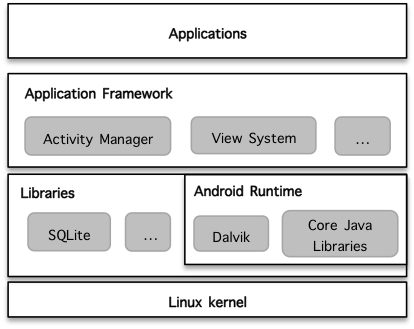
\includegraphics[scale=0.8]{arch3.png}
%  \caption{Android Architecture} \label{fig:exchier} \end{figure}

\subsection{Exception Model in Java} \label{sec:extypes}

\emph{\textbf{Exception Types.}} In Java, exceptions are represented according to a class hierarchy, on which
 every exception is an instance of the Throwable class, and can be of three kinds: the checked exceptions
(extends Exception), the runtime exceptions (extends RuntimeException) and errors
(extends Error)~\cite{gosling2000java}. Checked exception received their name
 because they must be declared on the method's \emph{exception interface} (i.e., the list of exceptions that a method 
might raise during its execution) and the compiler statically checks if
 appropriate handlers are provided within the system.
Both runtime exceptions and errors are also known as ``unchecked exceptions'', as 
they do not need to be specified on the method \emph{exception interface} and do not trigger any 
compile time checking.

By convention, instances of Error represent  unrecoverable conditions which usually result
from failures detected by the Java Virtual Machine due to resource limitations, such as OutOfMemoryError.
Normally these cannot be handled inside the application.  Instances of RuntimeException are implicitly 
thrown by Java runtime environment when a program violates 
the semantic constraints of the Java programming language (e.g., out-of-bounds array index, divide-by-zero 
error, null pointer references). Some programming languages react to such errors by immediately terminating the program, while
other languages, such as C++, let the program  continue
 its execution in some situations such as the out-of-bounds array index.
According to the Java Specification~\cite{gosling2000java} programs are not 
expected to handle such runtime exceptions signaled by the runtime environment. 

User-defined exceptions can be either checked
 or unchecked, by extending either Exception or RuntimeException. There is a long-lasting debate 
about the pros and cons of both approaches~\cite{javatut,stackoverlow,debate}
%\footnote{152 questions in Stackoverflow are related to this debate}. 
Section ~\ref{sec:best} presents
a set of best practices related to each of them.

%\begin{figure} \centering 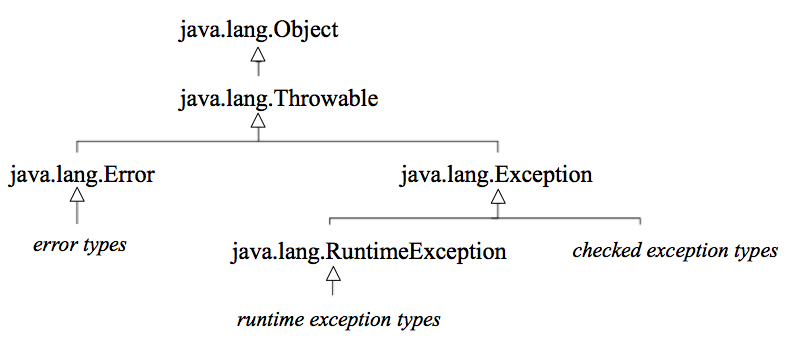
\includegraphics[width=\hsize]{new2_hierarchy.png}
% \caption{Exception Hierarchy in Java} \label{fig:exchier} \end{figure}

\emph{\textbf{Exception Propagation.}} In Java, once an exception is thrown, 
the runtime environment looks for the nearest enclosing exception handler
(Java's try-catch block), and unwinds the execution stack if necessary.
This search for the handler on the invocation stack aims at increasing software reusability, 
since the invoker of an operation can handle the exception in a wider context ~\cite{miller1997issues}.

 A common way of  propagating exceptions in Java programs is through exception wrapping
 (also known as exception chaining): One exception 
is caught and wrapped in another which is then thrown instead. Figure~\ref{fig:wrapping} shows 
an exception stack trace which illustrates such exception wrapping. 
For simplicity, in this paper we will refer to ``exception stack trace'' as as just stack trace.
The bottom part of the stack trace is the \emph{root exception}, which indicates
the first reason (root cause) for the exception thrown (in this case, the computer run out of
memory). The top part of the stack trace indicates the location of the exception
manifestation (which we will refer to as the \emph{exception wrapper} in this paper). The
execution flow  between the root exception and the wrapper may
include other intermediate exception wrappers. In all levels, the exception
\emph{signaler}, is the method that threw the exception, represented on the
stack trace as the first method call below the exception declaration.

\begin{figure} \centering 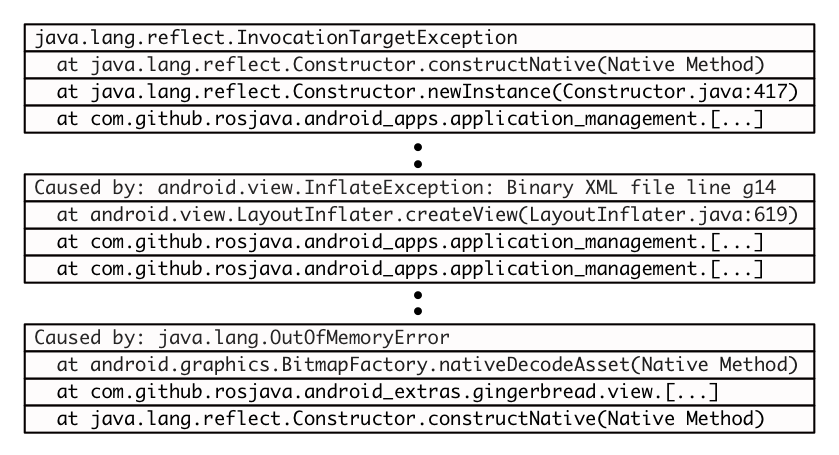
\includegraphics[scale=0.5]{stacktrace_bw.png}
\caption{Example of an exception stack trace in Java.}
\label{fig:wrapping}
\end{figure}

\subsection{Best Practices}
\label{sec:best}

Several general guidelines have been proposed on how to use Java
exceptions~\cite{mandrioli1992advances,gosling2000java,wirfs2006toward,
bloch2008effective}. Such guidelines do not
advocate any specific exception type, but rather propose ways to effectively use each of them.
Based on these, for the purpose of our analysis we compiled the following list of Java exception handling best practices.

%\noindent\emph{Meaning of Exception Types}

\emph{I-Checked exceptions should be used to represent recoverable
conditions} (\cite{mandrioli1992advances,gosling2000java,wirfs2006toward,bloch2008effective}).
The developer should use checked exceptions for conditions from which the caller
is expected to recover. By confronting the API user with a checked exception,
the API designer is forcing the client to handle the exceptional condition. The
client can explicitly ignore the exception (swallowing, or converting it to
another type) at the expense of the program's robustness~\cite{gosling2000java}.

\emph{II-Error represents an unrecoverable condition which should not be handled} 
(\cite{gosling2000java}).  Errors should result from failures detected
by the runtime environment which indicate resource deficiencies, invariant
failures or other conditions, from which the program cannot possibly recover.

%\noindent\emph{Exception Throwing}

\emph{III-A method should throw exceptions that precisely define the
exceptional condition} (\cite{gosling2000java,bloch2008effective}). To do so,
developers should either try to reuse the exception types already defined in the
Java API or they should create a specific exception. Thus, throwing general types such as a
pure java.lang.Exception or a java.lang.RuntimeException is considered bad practice.

%\noindent\emph{Exception Documentation}
%\textbf{IV- It is wise to document all exceptions thrown by a method} 

\emph{IV- All exceptions explicitly thrown by reusable code should be documented.}
(\cite{mandrioli1992advances,gosling2000java,wirfs2006toward,bloch2008effective}).
For checked exceptions, this is automatically the case.
Bloch~\cite{bloch2008effective} furthermore recommends to document explicitly thrown
run time exceptions, either using a throws declaration in the signature, or using
the @throws tag in the Javadoc.
Doing so, in particular for public APIs of libraries or frameworks,
makes clients aware of all exceptions possibly thrown,
enabling them to design the code to deal with them and use the API effectively~\cite{Robil00,wirfs2006toward}.



\section{Study Design}
\label{sec:study}


\begin{figure*} \centering 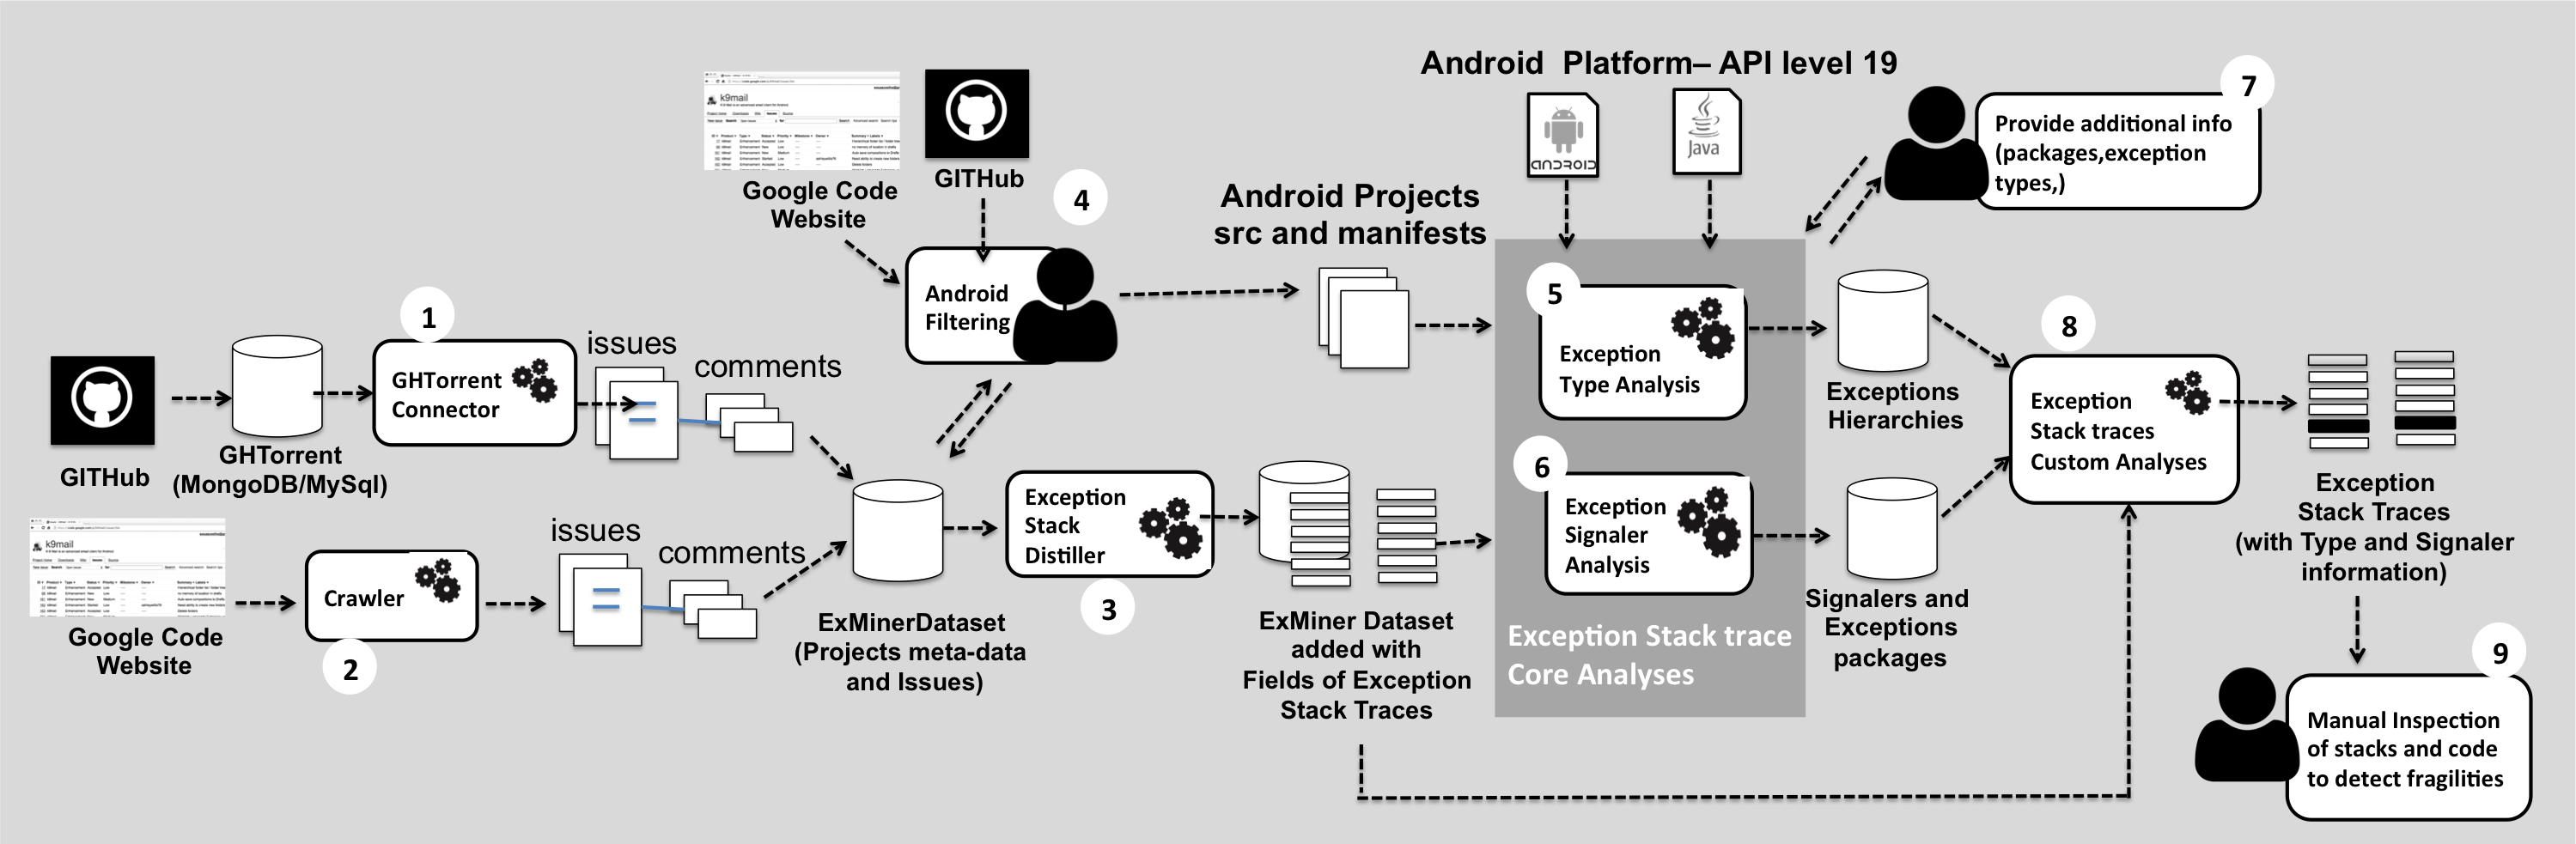
\includegraphics[scale=0.3]{studyoverview3.png}
\caption{Study overview.} \label{fig:overview} \end{figure*}

%This section describes the exploratory study whose goal was to investigate:
%\begin{description}
 % \item[RQ] \noindent\emph{Which fragilities on the exception-related code can be revealed from a post morten exception stack trace analysis of Android projects?} 
 %    \item
%\end{description}
%One major decision that had to be made for our investigation was the selection of the target 
%projects. We have selected a set of XXX open-source Android projects hosted in GitHub and 
%Google Code. GitHub and Google Code are among the most used hosting sites for open-source
 %projects,
% We investigate whether characteristics 
%of exception stack traces can pinpoint best practices violations and therefore reveal \emph{bug hazards}.

The goal of this exploratory mining study was to investigate whether the exception stack traces 
embedded on issues of Android projects (hosted in GitHub and Google Code), can reveal 
\emph{bug hazards} on the exception-related code of both the applications and the underlying framework. 
As mentioned before, in this context \emph{bug hazards} are the characteristics on the exception-related code 
that favor the introduction of failures such as uncaught exceptions. 

This exploration is guided by the set of best practices compiled in this study.
To support this investigation, we developed a tool called ExceptionMiner (Section~\ref{sec:exceptionminer})
which extracts the exception stack traces embedded on issues, 
and combines stack trace information with source code and bytecode 
analysis. Moreover, manual inspections were also used to leverage
 the understanding of stack traces and support further discussions and insights (Section~\ref{sec:manual}).

Figure~\ref{fig:overview} gives an overview of the study.
Firstly  the issues reported on Android projects hosted on GitHub and Google Code were recovered (Figure~\ref{fig:overview} - (1) and (2)).
Then the stack traces embedded each issue were extracted and distilled (Figure~\ref{fig:overview} - (3)).
The stack trace information were then combined with source code and bytecode analysis in order to discover 
the type of the exceptions reported on the stack traces (e.g., error, runtime, checked)  (Figure~\ref{fig:overview} - (5))  and the origin of such exceptions 
(e.g., the application, a library, the Android platform)  (Figure~\ref{fig:overview} - (6)). 
Manual inspection steps were used to support the mining process (Figure~\ref{fig:overview} - (4), (7) and (9)) and 
the search for \emph{bug hazards}  (Figure~\ref{fig:overview} - (8)). Next sections detail each step of this mining process.

Our study focused on open-source apps, since the information needed to perform our study
cannot be retrieved from commercial apps, whose issue report systems and 
source codes are not publicly available. The Android open-source apps were also 
target of other research studies ~\cite{Linar13,ahimed}.   
In this study we explore the domain quantitatively and highlight interesting cases by 
exploring cases qualitatively. 

%\subsection{Data Extraction Process}
%\label{sec:miningproc}

%In this exploratory study the following information is needed: (i) the issues reported on Android projects hosted on 
%GitHub and Google Code; (ii) the stack traces embedded on these issues; (iii) the type of the exceptions
 %reported on the stack traces (e.g., error, runtime, checked); (iv) the origin of such exceptions 
%(e.g., the application, a library, the Android platform). Next, we describe: how such information 
%was retrieved from GitHub and Google Code.

%mentioned 
%The data used in our study to answer our research questions are: the issues related to each 
%Android project available in each repository; the source code and manifest file of each application;
%the bytecode of all exceptions defined and reused by Android platform.

\subsection{Android Apps in GitHub}
\label{sec:git}


\begin{table}
  \centering
  \begin{tabular}{lr|lr}
    \hline
     \multicolumn{2}{c}{\bfseries{GitHub}} &  \multicolumn{2}{c}{\bfseries{Google Code}} \\
      \bfseries{Lable} &  \bfseries{\% Occurrences} &  \bfseries{Lable} &  \bfseries{\% Occurrences} \\
    \hline
empty &	54.24\% & Defect &	91.96\% \\
Defect &	39.56\%  & Enhancement  &	3.16\% \\
Enhancement &	0.57\% & Task	& 1.37\% \\
Support &	0.52\% & empty &	1.12\% \\
Problem &	0.36\% & StackTrace &	0.70\% \\
Others &	4.74\% &  Others &	1.68\% \\   
  \hline
  \end{tabular}
  \caption{Labels on issues including exception stack traces.}
  \label{tab:lables}
\end{table}

%As mentioned before, this study mined information available on GitHub issues,
%more specifically, extracting and distilling the stack traces embedded on GItHub issues. 

This study used the dataset provided by the GHTorrent project~\cite{Gousi13}, 
an off-line mirror of the data  offered through the Github API.  
To identify Android projects, we performed a case insensitive search for the
term ``android" in the repository's names and short descriptions.  
Up to 23 Feb 2014,  when we queried GHTorrent, such heuristic could
 find 2.542 repositories. Running the ExceptionMiner tool 
 in this set we observed that 589 projects had at least one issue containing a stack trace.
	
Then we performed further cleanup, inspecting the site of every Android project
reporting at least one stack trace, to make sure that they represented real
mobile apps. During this clean up 106 apps were removed because they were either
example projects (i.e., toy projects) or tools to support Android development
(e.g. Selendroid, Roboeletric - tools to support the testing of Android apps).
The filtered set consisted of 482 apps. This set of 482 projects contained overall 31,592 issues from which 4,042 exception stack traces 
were extracted. Issues on Github are different from issues on dedicated bug tracking tools such as 
Bugzilla and Jira. The most important difference is that there are no predefined fields
  (e.g. severity and priority). Instead, Github uses a more open ended tagging system, on which
repositories are offered a pre-defined set of labels, but repository owners can modify 
them at will. Therefore, an issue may have none or an arbitrary set of labels depending 
on which repository it was created. Table~\ref{tab:lables} illustrates the ocurrences of different labels 
on the issues including exception stack traces.

Based on the assumption that regardless the issue lables, every exception stack
trace contains relevant information concerning the exception structure of the
projects analyzed - and therefore can review \emph{bug hazards} on the exception-related code -  
we opted for not restricting the analysis only on defect issues.

%\footnote{We conducted the same analysis 
%on the defect issues only and the top exceptions were quite similar.
% Due to space limitation we limit to present the general analysis here. More detailed analysis
%on the defect issues can be found at:\url{https://github.com/souzacoelho/exceptionminer}}. 

\subsection{Android Apps in Google Code}
Google Code contains largely used open-source Android apps (e.g. K9Mail\footnote{K9Mail moved to Github but as a way of not loosing the project history it advises their users to report bugs on Google Code issue tracker: https://github.com/k9mail/k-9/wiki/LoggingErrors.}),
 however, differently from GitHub, Google Code does not provide an API to access the information related
 to hosted projects\footnote{Google code used to provided a Web service to such repository, but it was deactivated in June 2013 what Google called a `clean-up action".}.
To overcome this limitation we needed to implement a Web Crawler (incorporated in ExceptionMiner tool described next) that navigated 
through the web interface of Google Code projects extracting all issues and issue comments and storing in a relational database for later analysis.

To identify Android projects in Google Code, we performed a similar heuristic: we performed a case insensitive search 
(on Google Code search interface) for the term ``android". On January 2014, when we queried Google Code, such heuristic could
 returned a list of 788  projects. This list comprised the seeds sent to our Crawler .

The Crawler retrieved all issues and comments for these projects.
From this set, 724 projects defined at least 1 issue. Running the ExceptionMiner tool 
 in this set we observed that 183 projects had at least one issue containing an exception stack trace.
 Then we performed further cleanup (similar to the one described previously) inspecting the site 
of each project. As a result we could identify 157 Android projects.  This set contained overall 127,456 issues,
 from which 1,963 exception stack traces were extracted. Table~\ref{tab:lables} illustrates the ocurrences of different labels 
on the issues including exception stack traces. Differently from GitHub, in Google Code most of 
the issues were labled as ``Defect". However, based on the same assumption described for the GitHub repository
 we considered all issues reporting stacks (regardless its labels).

%SELECT distinct(type), count(*) as n
%  FROM exceptionalissue where repo !='android' group by type order by n desc;

%For instance: K9mail  was hosted in Google Code 
%before moving to GitHub and in order not to loose the project history it advices their 
%users to create issues on Google Code as a way to preserve project history.

%To overcome this limitation and mine the information available on such Google Code 
%projects we implemented a Web crawler which navigated (incorporated in ExceptionMiner tool described next) 
% on each project and issue page, extracting the content of each issue to store on relational database.

%{MOSTRAR UMA FIGURA COM TODOS OS PASSOS E RESSALTAR OS PASSOS MANUAIS}
%COMPLETE HERE.....
%\subsubsection{Database of Exception Stack Trace Information}
%\subsubsection{Distiling Exception Stack Trace Information}
%\subsection{Process}
%ESPALHAR ESTA SECAO NAS OUTRAS.
%Figure~\ref{fig:overviewfig} presents an overview of the mixed-methods approach
%conducted to answer these questions. The mixed-methods approach is composed by the following steps:

\subsection{The ExceptionMiner Tool}
\label{sec:exceptionminer}

The ExceptionMiner is a mining tool which can connect to different issue repositories, 
extract issues, mine exception stack traces from them, distill exception stack trace information,
and enable the execution of different analyses by combining exception stack 
trace information with bytecode and sourcecode analysis. The main components of ExceptionMiner are as follows:

\emph{\textbf{Repository Connectors.}} This component enables the connection 
with issue repositories. In this study two main connectors were created: one which connects to 
GHTorrent database, and Google Code connector which is comprised of a Web Crawler,
 that can traverse the Google Code web interface and extract the project issues. 
Projects meta-data and the issues associated to each project are stored on a relational 
database.

\emph{\textbf{Exception Stack Trace Distiller.}}
This component is based on a combination between a parser (based on regular expressions) 
and heuristics able to identify and filter exception names and stack traces inline with text. 
This component distills the information that composes a stack trace.
 Some of the attributes extracted from the stack trace are:
 the root exception and its signaler, the exception wrappers and their corresponding signalers. 
This component also distills fine grained information of each attribute such as: the classes and packages associated to them.
In contrast to existing issue parsing solutions such as Infozilla, the parser
created in this work can discover stack traces mixed with log information\footnote{In several 
exception stack traces, the exception frames were preceeded by logging information e.g., 
"03-01 15:55:01.609 (7924): at android.app.ActivityThread.access\$600(ActivityThread.java:127) 
"which could not be detected by existing tools.}.

\emph{\textbf{Exception Type Analysis.}} To support a deeper investigation of the 
stack traces every exception defined on a stack trace need to be classified according to its type
(e.g. Error, checked Exception or RuntimeException). The module responsible for this analysis 
uses Design Wizard~\cite{Brunet09} framework to inspect the bytecode of all exceptions reported on issues,
and a specific implementation to analyze the source code of Java Exception classes (when the
bytecode was not available). It walks up the type hierarchy of a Java exception until it reaches a base exception type.
This module analyzed all exceptions defined on Android platform (API level 19) - 
which includes all basic Java exceptions that can be thrown during the app execution,
and exceptions thrown by Android core libraries. Moreover, it also analyzed the 
exceptions reported on stack traces that were defined on applications and third-party libraries 
(the tool only analyzed the last version available).

\emph{\textbf{Exception Signaler Analysis.}}
This module is responsible for classifying each signaler according 
to its origin (i.e. Android Application Framework, Android Libcore, Application, Library). 
Table~\ref{tab:signalers} presents the heuristic adopted in this classification.
To enable such classification, we needed to feed this module with the information
comprising all Java packages that compose: the Android Plaform;
 the Android Libcore; and each analyzed Application. 
To discover the packages composing the first two origins
we could refer to the Android Specification.
To discover the packages composing each application, this module 
extracted the manifest files of each Android app
 - which defines the main packages that compose the applications.
 Whenever this file was not available, the tool recursively analyzed the 
structure of source-code directories composing the app
- filtering out the cases on which the application 
also included the source code of reused libraries.
Then, based on this information and using pattern matching 
between the signaler name and the packages, this module identifies 
the origin of the exception signalers. The exceptions were considered
 from libraries if their packages were neither defined 
on Android platform, nor on core libraries, nor on applications.
Table~\ref{tab:signalers} summarizes the signaler classification.

%\noindent\emph{Exception Wrapping Analysis.} 
%\noindent\emph{Concern Mapping.} 

\begin{table}
  \centering
  \begin{tabular}{rp{29em}}
    \hline
    \bfseries{Signaler} & \bfseries{Description} \\
    \hline
    \bfseries{android} & If the exception is thrown on a method defined in Android platform.\\
    \bfseries{app}     & If the exception is thrown on an method defined on an Android app.\\
    \bfseries{libcore} & If the exception is thrown on one of the core libraries reused by Android (i.e., org.apache.harmony, org.w3c.dom, sun.misc, org.apache.http, org.json, org.xml). \\
    \bfseries{lib}     & If the exception is thrown on a method that was not defined by any of the elements above.\\
    \hline
  \end{tabular}
  \caption{Sources of exceptions in Android}
  \label{tab:signalers}
\end{table}

\subsection{Manual Inspections}
\label{sec:manual}
In the context of the ExceptionMiner tool, manual inspections were used to:
(i) support on the identification of packages composing the Android platform, 
libs and apps analyzed in this study (as described previously); and (ii)  
identify the type of some exceptions reported on issues, 
that were not be automatically identified by the ExceptionMiner tool
(because they were defined on previous versions of libraries,
apps and Android Plaform). When the exception could not be  
found neither automatically, nor manually (because they were defined on a previous version
of the app or lib) the exception were classified 
in our study as ``Undefined".  Only 31 exceptions 
remained undefined - such exceptions were reported on 61 exception stack traces as 
presented in Table ~\ref{tab:typeroottab}.

\subsection{Replication Package}
All the data used in this study is publicly available at https://github.com/souzacoelho/exceptionminer.
Specifically we provide: (i) all issues related to Android projects found
in GITHub and Google Code used in this study; (iii) all stack traces extracted
from issues (ii) the results of manual inspection steps; (iv) the tool developed 
in this work to support stack trace extraction and distilling.

\section{The Study Results}
\label{sec:result}

This section presents the results of the study, providing both a
quantitative and qualitative analysis of the outcomes. The structure of this section
 is centered on questions that guided the search for \emph{bug hazards} on the exception-related code
based on exception stack trace information.

\subsection{What can the Common Root Exceptions tell us? }

After distilling the information available on the exception stack traces, we could find 
the exceptions commonly reported as the root causes of stack traces.
Table \ref{tab:topten} presents a list of the top 10 root exceptions found in the study - 
 ranked by the number of distinct projects on which they were reported. 
This table also shows how many times the signaler of such exception was a method defined on
the Android platform, the Android libcore, the application itself or a third-party library -
 following the classification presented in Table  \ref{tab:signalers}. 

\begin{table*}
  \centering
  \begin{tabular}{rcccccccc}
    \hline
    \bfseries{Root Exception} &  \multicolumn{2}{c}{\bfseries{Projects}} &  \multicolumn{2}{c}{\bfseries{Occurrences}} & \textsf{Android} & \textsf{Libcore} & \textsf{App} & \textsf{Lib} \\
    & \bfseries{\#} &  \bfseries{\%} & \bfseries{\# } & \bfseries{\% } &&&&\\
    \hline

java.lang.NullPointerException	&	332	&	51.96\%	&	1664	&	27.71\%	&	525	&	20	&	836	&	280	\\
java.lang.IllegalStateException	&	120	&	18.78\%	&	278	&	4.63\%	&	185	&	31	&	41	&	39	\\
java.lang.IllegalArgumentException	&	142	&	22.22\%	&	353	&	5.88\%	&	195	&	12	&	95	&	44	\\
java.lang.RuntimeException	&	122	&	19.09\%	&	319	&	5.31\%	&	203	&	2	&	64	&	51	\\
java.lang.OutOfMemoryError	&	78	&	12.21\%	&	237	&	3.95\%	&	141	&	16	&	35	&	34	\\
java.lang.NoClassDefFoundError	&	67	&	10.49\%	&	94	&	1.57\%	&	10	&	0	&	46	&	37	\\
java.lang.ClassCastException	&	64	&	10.02\%	&	130	&	2.16\%	&	55	&	0	&	55	&	20	\\
java.lang.IndexOutOfBoundsException	&	62	&	9.70\%	&	166	&	2.76\%	&	53	&	0	&	93	&	18	\\
java.lang.NoSuchMethodError	&	54	&	8.45\%	&	80	&	1.33\%	&	10	&	0	&	56	&	14	\\
java.util.ConcurrentModificationException	&	43	&	6.73\%	&	65	&	1.08\%	&	5	&	0	&	46	&	13	\\
    \hline
  \end{tabular}
\caption{Root Exceptions occurrences and popularity in repositories hosted in Google Code (GC) and GitHub(GH).}
\label{tab:topten}
\end{table*}

%\begin{figure}
%\centering
%\includegraphics[width=\hsize]{top_exceptios_android_new2.pdf}
%\includegraphics[width=\hsize]{top_exceptions_android_new}
%\caption{Top exceptions in Android repositories.}
%\label{fig:androidsignaler}
%\end{figure}
 
We can observe that most of the exceptions on this list are implicitly thrown by the
 runtime environment due to programming mistakes  (e.g., out-of-bounds array index, division-by-zero, access to a null reference)
 or resource limitation (e.g., OutOfMemoryError). 
From this set the java.lang.NullPointerException was the most reported root cause (27.71\%). 
If we consider the frequency of NullPointerException 
across projects, we can observe that 51.96\% of all projects reported at least one exception stack 
trace on which the NullPoiterException was the root cause.

 The NullPointerException was mainly signaled inside the application code (50\%) and the Android platform (31.5\%),
 although we could also find the NullPointerException being signaled by third-party libraries (16.3\%). 
Regarding reusable code (e.g., libraries and frameworks), there is no consensus whether it is a good or a bad practice to 
re-throw a NullPointerException. Some prefer to encapsulate such an exception on
an instance of IllegalArgumentException, while others~\cite{bloch2008effective} argue that the
NullPointerException makes the cause of the problem explicit and hence 
should not be wrapped.

The high prevalence of NullPointerException is aligned with the findings of other research
works~\cite{kim2013predicting,fraser20131600,csallner2004jcrasher,kechagia2014}. For instance, Sunghun et
al.~\cite{kim2013predicting} showed that 38\% the bugs related to exception handling in Eclipse project
 were caused by NullPointerException; Kechagia and Diomidis showed that NullPointerException was the  
most reported exception on the crash reports sent to BugSense (a bug report 
management service for Android applications); 
other works on robustness testing~\cite{maji2012empirical,csallner2004jcrasher} showed that most of the automatically 
detected bugs were due to NullPointerException and exceptions implicitly-signaled by Java 
environment due to programming mistakes or resource limitations
 (as the ones found in our study).


%Commented 2015
%\emph{\textbf{The prevalence of programming mistakes on stack traces.}} 
%One way of getting a broader view of the prevalence~\footnote{The prevalence
 %evaluates the proportion of a given characteristic over a group 
%of subjects.}  of programming mistakes on reported stack traces would be to manually 
%inspect the code responsible for throwning every exception reported  on issues. 
%However, inspecting the source code related to %6005 stack traces can %easily become infeasible.
%Hence, we conducted an empirical investigation based on the following assumption: the name of the exception and its associated Javadoc 
%documentation hold enough information to pinpoint a ``programming mistake".To exemplify, an instance of ArrayOutOfBoundException
%pinpoints to programming mistake which indicates that an array has been accessed with an illegal index.

%To perform this empirical investigation, we selected a subset of all reported root exceptions. 
%This subset was composed by the top 100 root exceptions (from a list ranked by the number of ocurrences on stacks).
%This subset was representative since it contained root exceptions that were reported as the root causes of 95\% of 
%all stack traces. Therefore, based on the inspection of the full names exceptions and the associated 
%Javadocs we could identify from this subset, which exceptions were related to programming mistakes.
% It is worth mentioning that  all exceptions identified as programming mistakes were exceptions defined on java.lang and java.util packages. 
%After doing such analysis, we could calculate the prevalence of such exceptions on issues. In other words, we could calculate the proportion of issues %mentioning the exceptions identified in this analysis as related to %``programming mistakes".

%Table ~\ref{tab:causes} summarizes the results. It also illustrates the number of general Java exceptions - 
%whose full name does not carry the reason for the exception to be thrown.
%To ensure the quality of the analysis, three independent developers classified a randomly selected
%sample of 25 exception types (from the total 100) using the same list of concerns;
%the resulting interrater agreement was high (96\%). 

%The results show that the programming mistakes are associated to the most reported root causes. 
%Although there is usually no proper handling for such exceptions~\cite{wirfs2006toward}, 
%besides presenting an error message to the user and restarting the application~\footnote{Only 
%high fault tolerant systems need to provide solutions to handle them.}.  
%This finding calls the attention to the following: the high number of programming mistakes reported 
%on issues are an indication that developers may be underestimating the impact that such 
%mistakes have on application robustness.

%\begin{table}
 % \centering
 % \begin{tabular}{lr}
 %   \hline
 %   \bfseries{Cause} &  \bfseries{\% Occurrences} \\
 %   \hline
 %     Programming Mistakes &  51.96\%\\ 
 %     %Memory Restriction   &   4.10\% \\ 
 %     General Exceptions   &  6.70\%\\
 %   \hline
% \end{tabular}
%  \caption{Identifying the concerns related to root exceptions}
%  \label{tab:causes}
% \end{table}


%\noindent \fbox{ \begin{minipage}{0.96\columnwidth} \emph{
%The study revealed: approximately 52\% of the reported stack traces were associated to programming mistakes;
%and 27.71\% of all stack traces reported a java.lang.NullPointerException as the root cause.
%}
%\end{minipage}}

\emph{\textbf{Identifying the Concerns Related to Root Exceptions.}} To get a broader view of the root exceptions of stack traces,
we performed an empirical evaluation whose goal was to identify the concerns related to the most reported root exceptions.
Besides the exceptions related to programming mistakes mentined before, we also looked for exceptions related to some concerns that are known as sources of faults in mobile development: concurrency ~\cite{ama2012} backward compatibility ~\cite{McDon13}, security ~\cite{enck2011study,was2010} and resource management (IO, Memory, Batery) ~\cite{Zhang12}.

Since it is infeasible to inspect the code responsible for throwning every exception reported in this study,
the concern identification of each exception was based on meaning of the exception type - defined on 
its Javadoc documentaion and on the Java specification. To exemplify: (i) an instance of ArrayOutOfBoundException  
refers to a programming mistake according to its Javadoc; and (ii) the Java specification lists all 
exceptions related to backward compatibility issues~\cite{javaback} (e.g., InstantiationError, VerifyError, IllegalAccessError).

To perform such mapping, we selected a subset of all reported root exceptions. This subset was composed by 100 root exceptions
which were reported on 95\% of all stack traces analyzed in this study. Hence, based on the inspection of the 
Javadoc related to each exception and Java specification, we identified the concern releated to each root exception. 
Table~\ref{tab:tophundrend} illustrates the result of this empirical evaluation. This table also illustrates the exceptions 
that could not be directly mapped to one of the aforementioned concerns, either because they were too general (i.e., java.lang.Exception,
java.lang.RuntimeException, java.lang.Error) or because they were related to other concerns (e.g., specific to an application or given library).

\begin{table}
\centering
\begin{tabular}{lrr}
\hline
\bfseries{Concern} & \bfseries{\% Occurrences on stacks} \\
\hline
Programming logic (java.lang and util) & 52,0\%\\
Resources (IO, Memory, Batery) & 23,9\% \\
Security & 4,1\%\\
Concurrency & 2,9\% \\
Backward compatibility & 5,5\% \\
Specific Exceptions & 4,9\%\\
General (Error, Exception, Runtime) & 6,7\%\\
\hline
\end{tabular}
\caption{Identifying the concerns related to root exceptions}
\label{tab:tophundrend}
\end{table}

To ensure the quality of the process, three independent coders classified a randomly selected
sample of 25 exception types (from the total 100) using the same list of concerns;
the interater agreement was high (96\%).
We can therefore assume that the categories are descriptive
enough for covering the range of exception types analyzed.

%These study showed that the programming mistakes associated to the most reported root causes.
%However, they may be interactly related to one of the other concerns. For instance, a concurrency problem may
%lead to a NullPointerException.


%For instance, the Java specification list all exceptions related to backward compatibility
%issues ~\cite{javaback} (e.g., InstantiationError, VerifyError, IllegalAccessError). 
%were also investigated in this study

\noindent \fbox{ \begin{minipage}{0.96\columnwidth} \emph{
A multitude of programming mistakes were reported as the main causes of exception stack traces.
52\% of all projects reported at least one exception stack trace on which the NullPoiterException
was the root cause.
}
\end{minipage}}

\subsection{What can the Exception Types tell us?}
%\subsection{Exploring the Information Embedded on Exception Types}
%\subsection{The Exception Types and What They can Tell us? }

As mentioned before, using the ExceptionMiner tool in combination with manual inspections we could identify
the root exception types (i.e., RuntimeException, Error, checked Exception) as well as its origins - which were 
identified based on the package names of the signalers related to it on the stack traces (Section~\ref{sec:exceptionminer}).
Table~\ref{tab:typeroottab} presents the types and origins of root exceptions of all analyzed stack traces. 

We can observe that most of the reported exceptions were runtime 
(64.85\%); and most of them were signaled by methods defined either on the Application (47.3\%)
or on the Android platform (34.3\%). We could also find runtime exceptions thrown by library code (17.7\%).
 
We can also see, from Table ~\ref{tab:typeroottab}, that contrasting with the other origins, most of the 
 exceptions signaled on Android Libcore (i.e., the set of libraries reused by the Android) were 
checked exceptions. Such set comprises: org.apache.harmony, org.w3c.dom, sun.misc, 
org.apache.http, org.json, org.xml, javax. Signaling checked exceptions is considered a 
good practice (see best practice IV in Section~\ref{sec:best}) because by using 
checked exceptions a library can define a precise 
\emph{exception interface} ~\cite{miller1997issues} to its clients.
 Since such libraries are heavily used  in several projects, such finding can be related to the libraries maturity.

%SELECT COUNT(*) FROM STACKTRACESUMMARY WHERE
% repo !='android'  AND MAIN_EXTENDS LIKE 'RUNTIME%' 
%SELECT COUNT(*) FROM STACKTRACESUMMARY WHERE
%repo !='android'  AND MAIN_EXTENDS LIKE 'RUNT%' AND MAINSIGNALER_FROM like 'APP%';

\begin{table}
\centering
\begin{tabular}{lccccrr}
    \hline
    \bfseries{Root Type} & \bfseries{Android} & \bfseries{Libcore} & \bfseries{App} & \bfseries{Lib}  & \bfseries{All} & \bfseries{\%} \\
    \hline

Runtime	&	1335	&	73	&	1843	&	690  &	3894 & 64.85\% \\  %2466+854
Error	       &	 188              &	 46	&	302             &	167	           &	691 & 11.51\%	\\
Checked	&	276           &	314	&	313          &	567	           &	1358 & 22.61\%	\\
Throwable	&	0	       &	0	&	2            &	0         &	2 & 0.03\%	\\
Undefined	&	4	&	0	&	18		&	38	   &	60	& 1.00\% \\
 \hline
All		& 1  803	&	433	&	2478	&	1462	&	6005 	\\
    \hline
  \end{tabular}
\caption{Types of root exceptions.}
  \label{tab:typeroottab}
\end{table}



\emph{\textbf{Inspecting Exception Interfaces.}}  According to the best practices mentioned before, 
 \emph{explicitly thrown} runtime exceptions 
should be documented as part of the \emph{exception interface} of libraries/framework reusable
methods. To investigate the obedience to such practice, we firstly filtered out all the exceptions implicitly
 signaled by  runtime environment (due to programming mistakes) - since these exceptions 
should not be documented on the method signature.  Then we inspected the code each method 
(defined either on Android  Aplication Framework or on third-party libraries) 
explicitly signaling a runtime exception.

Table~\ref{tab:runtimeinterface} presents the results of this inspection. 
We could find 79 methods (both from libraries and Android platform) that  explicitly threw a runtime exception 
without listing such exception on the \emph{exception interface} (i.e., using 
throws clause on method signature). From this set only one method (defined on a library)
included an @throws tag on Javadoc - reporting that the given runtime exception
could be thrown in some contidions. These methods were responsible for 
267 exception stack traces mined in this study.

This result is aligned with the results of other two studies ~\cite{sacramento2006unchecked,kechagia2014}. 
One conducted by  Sacramento et al ~\cite{sacramento2006unchecked} - which observed that the
runtime exceptions in .Net programs are most often not documented. And other conducted by 
Kechagia and Spinellis ~\cite{kechagia2014} which discovered a set of methods 
on the Android API which do not documented runtime exceptions. One limitation 
of the work of Kechagia and Spinellis is that it did not filter out exceptions that,  
although runtime, should not be documented because they were implicitly signaled by the 
JVM due to resource restrictions or violations on Java semantic constraints.

When explicitly signaling a runtime exception and not documenting it, 
the developer imposes a threat to system robustness, specially
when such exceptions are thrown by a third party code (e.g. libraries, or framework utility code)
 invoked inside the application. In such cases the developer usually does not have access to 
the source code. Hence in the absence of the exception documentation it is very difficult or even impossible
 for the client to design the application to deal with ``unforeseen" runtime exceptions. As a consequence, the
 undocumented runtime exception may remain uncaught and lead to system crashes.

\noindent \fbox{ \begin{minipage}{0.96\columnwidth} \emph{
The study revealed: 267 exception stack traces were caused by ``undocumented runtime exceptions" 
thrown by libraries or the Android platform.
}
\end{minipage}}


\begin{table}
\centering

 %\begin{tabular}{|p{7.9cm} p{0.1cm}|}
\begin{tabular}{lrrrr}
    \hline
 \bfseries{Origin}   &  \bfseries{stacks}  & \bfseries{signaler methods} &  \bfseries{throws clause}  &  \bfseries{\@throws}  \\ 
\hline					
Libraries	& 	205	 & 	44	& 0	& 1	\\
Android  	&	62 &	35	&0 &  0	\\					
\hline					
\bfseries{All}	&	267 &	79 &  0  & 1\\
\hline					
  \end{tabular}
\caption{Absence of exception interfaces on methods.}
\label{tab:runtimeinterface}
\end{table}


\emph{\textbf{On the Presence of Checked Exceptions on Exception Interfaces.}} 
In this study, the exception stack trace analysis revealed an unexpected bug hazard: a 
checked exception thrown by a native method and not declared on the exception 
interface of these methods signaling them. Such native method was defined on
 the Android platform -  which uses Java Native Invocation (JNI) to access 
native C/C++ code. This exception was thrown by the method getDeclaredMethods defined in java.lang.Class. 
The Java-side declaration of this method does not have any throws clause, 
leading programmers and the compiler to think that no checked exceptions can be thrown.
 However, the C-code implementation did throw a ``checked exception" called NoSuchMethodException, 
violating the declaration. The Java compiler could not detect this violation, because it does 
not perform static exception checking on native methods. This type of bug is hard to diagnose
because the developer usually do not have access to the native implementations. 
Consequently, since it is not expected by the programmer, when such method throws 
this exception, such undocumented exception may remain
uncaught and cause the app to crash, or may be mistakenly handled by subsumption.
The exception stack traces reporting this scenario is actually a real bug of Android 
Gingerbread version (which still accounts for 13.6\% of devices running Android).
%Among the Android projects on which this exception stack trace was reported we can cite:
%PageTurner (206 stars), ActionBarSherlock (6,041 stars), otto (1,618 stars).

\noindent \fbox{ \begin{minipage}{0.96\columnwidth} \emph{
The study revealed: a checked exception being thown by a native method and not declared  
on the \emph{exception interface} of such method and all methods on the invocation chain.
}
\end{minipage}}


\subsection{What can the Exception Wrappings tell us?}


\begin{table}
\centering

 %\begin{tabular}{|p{7.9cm} p{0.1cm}|}
\begin{tabular}{ll}
    \hline
 id & \bfseries{Runtime wrapping Error}    \\  %\bfseries{\#}
    \hline
1 & java.lang.RuntimeException - java.lang.OutOfMemoryError  \\ %30
2& java.lang.RuntimeException -  java.lang.StackOverflowError)   \\ %4
\hline
& \bfseries{Checked wrapping Error}  \\
 \hline
3&java.lang.reflect.InvocationTargetException - java.lang.OutOfMemoryError  \\ %5
4&java.lang.Exception - java.lang.OutOfMemoryError   \\ %1
\hline
& \bfseries{Error wrapping Checked}  \\
 \hline
5&java.lang.NoClassDefFoundError - java.lang.ClassNotFoundException   \\ %4
6&java.lang.AssertionError - javax.crypto.ShortBufferException)   \\ %3
\hline
& \bfseries{Error wrapping Runtime}    \\
 \hline
7&java.lang.ExceptionInInitializerError - java.lang.NullPointerException   \\ %9
8&java.lang.ExceptionInInitializerError - java.lang.IllegalArgumentException 	 \\ %2
 \hline
  \end{tabular}
\caption{Examples of Cross-type wrappings}
\label{tab:exampeswrap}
\end{table}


\begin{table*}
  \centering
  \begin{tabular}{llcccccc}
    \hline
    \bfseries{Wrapper Type}  &  \bfseries{Root Cause Type} &  \bfseries{Projects}  &  \bfseries{Occurrences} & \textsf{Android} & \textsf{Java/Libcore} & \textsf{Lib} & \textsf{App}  \\
    \hline
      
      Runtime &  Checked   & 88 & 148 &  75 &  0   & 38 &  35 \\  %(50.7\%) 
      Runtime   &  Error      & 46  &  67    &  58  &  0   & 8  &  1   \\      %(86.5\%) 
      Checked &  Runtime   & 17  & 31 & 4 &  0  & 16  &  11 \\  %(51.6\%) 
      Checked & Error         & 8    &  9  & 5  &  0  &  1 &  3  \\
      Error & Checked         & 14  &  27 &  6  &  7  &  6 &   8    \\
      Error & Runtime        & 8      &  17   & 1 &  1  & 1 &  14    \\

  \hline
      %none   & Runtime   &  2360 & 359 \\
      %none  &   Checked  & 422  & 117 \\
      %none  &   Error   & 381  & 141 \\
      %none &  Undefined  &  15   & 10  \\
      %none & Throwable  &  1    & 1 \\
     %\hline
      %Runtime   & Runtime & 560  & 182 \\    
      %Checked   & Checked & 98   & 42  \\
      %Error     & Error   & 15   & 14  \\
    %\hline
  \end{tabular}
\caption{Wrappings comprising different exception types.}
\label{tab:wrappingandroid}
\end{table*}

Java is the only language that provides a hybrid exception model 
which offers three kinds of exceptions each one holding an intended exception behavior (i.e., error, 
runtime and checked). Table~\ref{tab:wrappingandroid} presents the wrappings found in this study that
include different exception types (i.e., Error, checked Exception and Runtime). We call 
such a wrapping a ``cross-type wrapping". Next we exemplify some of such
 wrappings and discuss whether some of them may impact the system robustness.

\emph{\textbf{Runtime Exception wrapping Error.}} From Table~\ref{tab:wrappingandroid}, we could observe that most of such wrappings
were performed by Android platform (50.7\%).
The code snippet below was extracted from Android and shows a general catch clause 
that converts any instance of Throwable (signaled during the execution
of an asynchronous task) into an instance of RuntimeException and re-throws it.  
Table~\ref{tab:exampeswrap} presents exceptions wrapped in this code snipet.  
Such wrappings mask an unrecoverable Error on a general runtime exception.

{\footnotesize
\begin{verbatim}
   try {
      ...
   } catch (InterruptedException e) {
      android.util.Log.w(..., e);
   } catch (ExecutionException e) {
      throw new RuntimeException("...",e.getCause());
   } catch (CancellationException e) {
      ...
   } catch (Throwable t) {
     throw new RuntimeException("...", t);
   }
\end{verbatim}
}

\emph{\textbf{Runtime wrapping Checked Exception.}} This wrapping was responsible for 49.5\% of
the cross-type wrappings.  From this set 50\%  were performed on methods defined on Android platform. 
We observed that it was a common implementation practice in the methods of Android platform.
However, using such general exception, is considered a bad practice according to Java specification 
and compiled guidelines, because it loses contextual information about the exception.

\emph{\textbf{Checked Exception wrapping Error.}} Most of these wrappings
 were also caused by the reflection library used by applications' methods. The methods responsible for the wrappings
were also native methods written in C. Table~\ref{tab:exampeswrap} illustrates
some of these wrappings some of them are masking an OutOfMemoryError
into a checked exception. Such wrappings may also mask an unrecoverable error
and may lead to the ``exception confusion problem" described next.

\emph{\textbf{Error wrapping Runtime and Checked Exceptions}} Table~\ref{tab:exampeswrap}  illustrates
examples of instances of Error wrapping instances of RuntimeException. A
lthough such wapping mixes different exception types,
since there is no obligation associated to handling runtime exceptions, such wrapping 
does not violated the aforementioned best practices. On the other hand, the inspection 
also revealed instances of Error wrapping checked exceptions. Such wrappings were 
mostly performed by Java static initializers. If any exception is thrown in the context of a static initializer 
(i.e., static block)  it is converted into an ExceptionInitializerError 
on the point where the class is first used.  Table~\ref{tab:exampeswrap} also illustrates
examples of such wrappings. Although such wapping may represent a design decision,
it violates the best practice related to checked exceptions and errors as it mix the intended handling 
behaviour associated to both types.

We could also observe that some stack traces included successive cross-type wrappings, 
such as: Runtime - Checked - Runtime - Checked - Runtime - Checked - Runtime. Hence, although some of these wrappings may be a result of design decisions, the mis-use of exception wrapppings may make the exception handling 
code more complex (e.g., the multiple wrappings) and error-prone,
 and lead to what we call ``exception confusion problem". To illustrate this problem we can use one of the wrappings discussed above.
When the developer is confronted with a checked exception, the designer of the API is telling him/her 
to handle the exceptional condition (according to Java Specification and 
best practices). However, such exception may be wrapping an Error such as OutOfMemoryError (which indicate resource deficiency 
that makes impossible for the program to recover). Hence, trying to handle such exception  
may lead the program to an unpredictable state.

\noindent \fbox{ \begin{minipage}{0.96\columnwidth} \emph{
The cross-type wrappings is an indication that even if the developer sticks to Java
specification and best practices, it may be dificult for her/him to prevent the code from 
incurring into situations that lead the program to an unpredictable state - 
e.g., when handling checked Exceptions that are `hiding" Errors.
}
\end{minipage}}


\section{Further Discussions}
\label{sec:disc}

%\begin{figure*} \centering 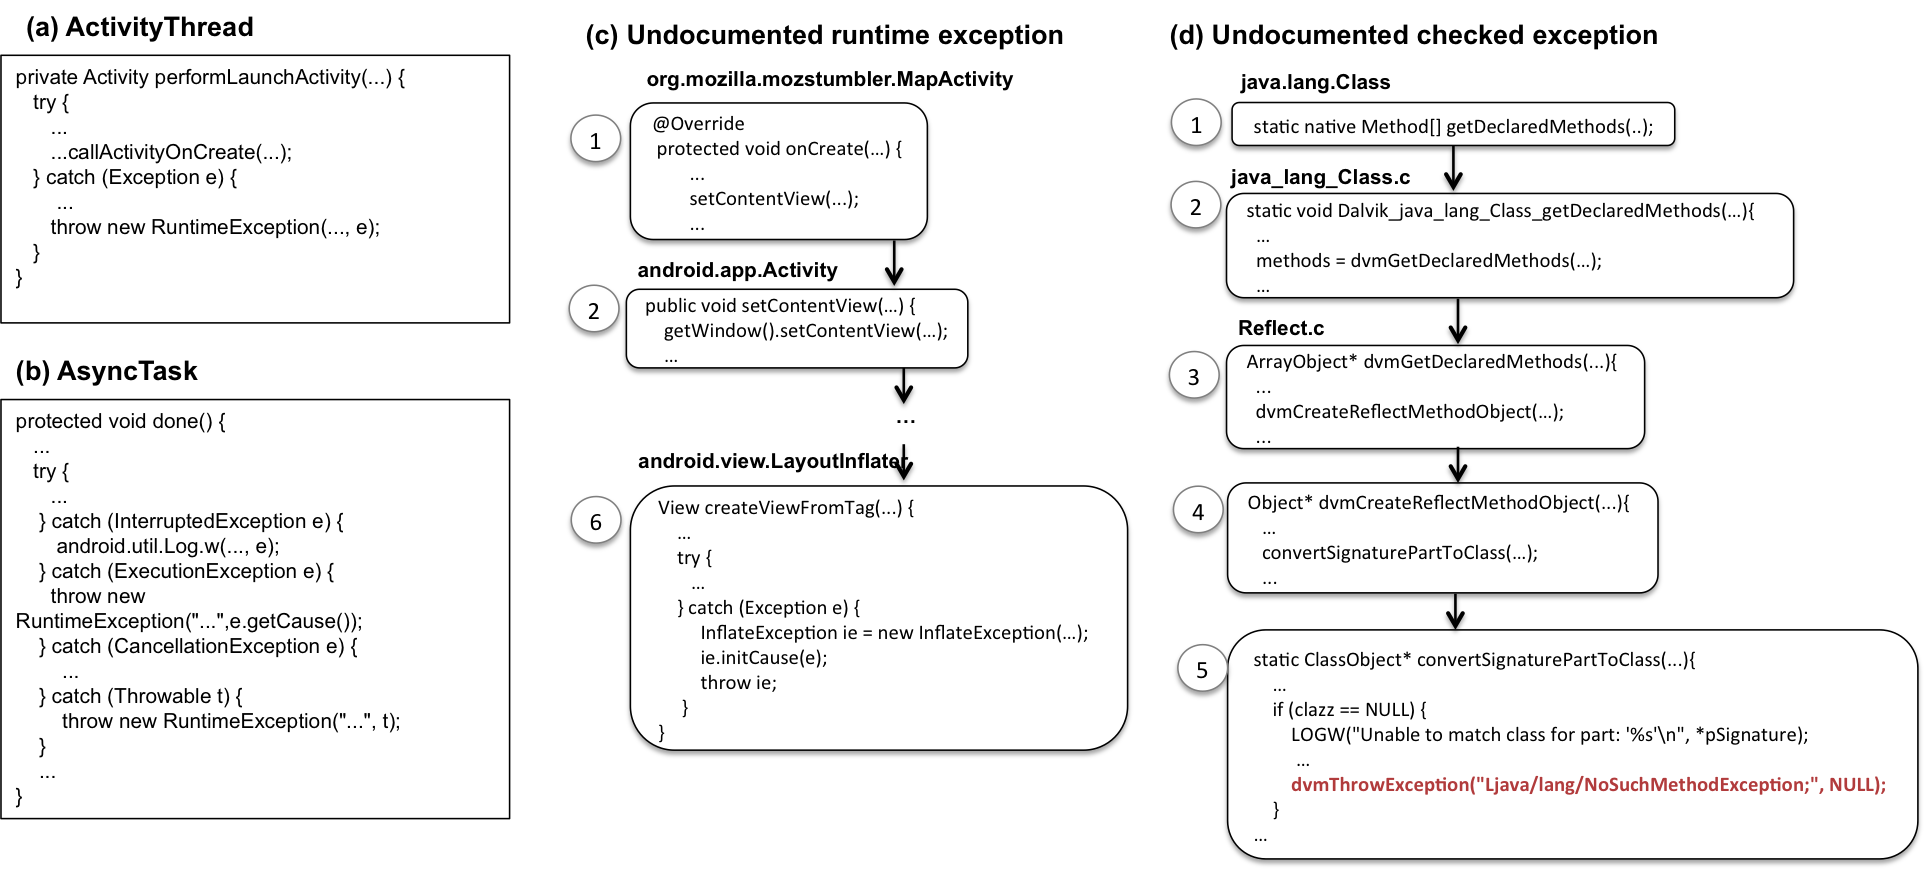
\includegraphics[scale=0.55]{examples_new2.png}
%\caption{Code snippets illustrating fragilities on the exception-related code} \label{fig:snippets} \end{figure*}

 ``Everybody hates thinking about exceptions, because they are not supposed to happen"
  (Brian Foote)~\footnote{Brian Foote shared his opinion in a conversation with James Noble - quoted on the paper: hillside.net/plop/2008/papers/ACMVersions/coelho.pdf}


\emph{\textbf{The exception handling confusion problem.}}
When (mis)applied, the exception wrapping can make the exception-related code
 more complex and lead to what we call an \emph{exception handling confusion problem}.
Such problem can lead the program to an unpredictable state in the presence of exceptions,
as illustrated by the scenario on which a checked exception wrapped an OutOfMemoryError. 
Currently there is no way of enforcing Java exception type conventions during program development.
Hence, further investigation is needed on finding ways to help developers in dealing with such
 problem, either preventing odd wrappings or enabling the developer to better deal with them or even
empirical studies on the real usefulness of Java hybrid exception model. 

%The cross-type wrappings detected in this study points to the fact that: (1) exception 
%wrappings may prevent exception types from being used according to its initial purpose
%(e.g, Errors should represent situations that should not be handled); and (2) may have been
% used to bypass the language restrictions imposed by checked exceptions  (e.g,
% checked exceptions may be wrapped in runtime exceptions).

\emph{\textbf{On the null pointer problem.}}
The null references was firstly introduced by Tony Hoare in ALGOL W, which after some years he called his ``one-billion-dollar mistake"~\cite{hoare2}.
In this sudy, the null references were, infact, responsible for several reported issues - providing more evidences to Hoare's speech.
This observation emphasizes the importance of solutions to avoid NullPointerExceptions, such as:
(i) lightweight intra-method null pointer analysis supported by Java8 @Nullable annotations~\footnote{They are used by tools e.g., Eclipse, IntelliJ, Android Studio 0.5.5 (release Apr. 2014) to detect potential 
null pointer dereferences at compile time.};
(ii) inter-method null pointer analysis tools such as the one proposed by Nanda and Sinha ~\cite{nanda2009accurate};
or (iii) language designs which avoid null pointers, such 
as Monads ~\cite{Walde95} (i.e., used in functional languages for values that may not be available 
or computations that may fail) could improve the robustness of Java programs. 

\emph{\textbf{On the need of rescues to the almost infeasible task of preventing uncaught exceptions}}
In this study we could observe undocumented runtime exceptions thrown by third party code,
and even undocumented checked exception thrown by a JNI interface.
Such undocumented exceptions make difficult, and most of the times infeasible
for the client code to protect against `unforeseen" situations that may happen 
while calling a library code. One may think that the solution for the uncaught exceptions may be to define a general handler, 
which is responsible for handling any exception that is not
adequately handled inside the applications. Although this 
solution may prevent  the system of abruptly crashing,
 such general handler will not have enough
contextual information to adequately handle the exception, 
a possible handler task is: to present a message to the user
 and restart the application. However, such handler cannot replace a carefully designed exception 
handling policy ~\cite{Robil00}, which can hardly be designed in the absence of 
third-party documentation on the exceptions that
may the thrown by it. On the other hand, documenting runtime exceptions is a tedious and error prone task, to help developers
mitigate this problem tools should be developed to automate the documentation of runtime exceptions
scraping from library code, few solutions in this directions have been proposed so far ~\cite{van2005combining}. 


\section{Threats to Validity}
\label{sec:threats}

%\noindent
\emph{Internal Validity.} We used a heuristics-based parser to mine
exceptions from issues.  Our parsing strategy was conservative by default; for
example, we only considered exception names using a fully qualified class name
as valid exception identifiers, while, in many cases, developers use the
exception name in issue description. Conservative parsing may minimize false
positives, which was our initial target, but also tends to increase false
negatives, which means that some cases may have not been identified as
exceptions or stack traces. Our limited manual inspection did not reveal such
cases. Moreover, in this study we manually mapped the concerns related to exceptions.
 To ensure the quality of the analysis, we calculated the interrater agreement after three independent 
developers classified a randomly selected sample (of 25 exception 
types from the total of 100); the interater agreement was high (96\%). 
Another threat relates to the fact that parts of our analysis 
are based on the availability of stack traces on issues reported on Github and Googlecode projects. 
In using these datasets, we make an underlying assumption: the stack traces reported on issues are 
representative of valid crash information of the applications. 
One way to mitigate such threat would be to access to the full 
set of crash data per application. Although some services exist 
to collect crash data from mobile applications ~\cite{BugSe14,BugSn14,Googl14,Acra14},
they do not provide open access to the crash reports of their client applications.
In our study, we mitigated this threat by manually inspecting
the source code associated to a subset of the reported exception stack traces.
Such subset comprises the stack traces related to the main findings 
of the study (e.g., ``undocumented runtime and checked exceptions",
and cross-type wrappings").
%\noindent

\emph{External Validity.} Our work uses GHTorrent dataset; although 
comprehensive and extensive is not an exact replica of Github. 
However, the result of this study does not depent on the analysis of
a complete Github dataset. Instead, the goal of our study was to 
pinpoint \emph{bug hazards} on the exception-related code based on 
exception stack trace mining of a subset of projects.
We limited our analysis to a subset of existing open-source Android projects.
We are aware that the exception stack traces reported 
for commercial apps can be different from the ones found in this study, and that
this subset is a small percentage of existing apps.
Such threats are similar to the ones imposed to other empirical studies 
which also used free or open-source Android apps ~\cite{Linar13,McDon13,ahimed}.
Moreover, several exception stack traces that support the findings of this study
refered to exceptions coming from methods defined on Android Application Framework
and third-party libraries.  Additionaly,  the \emph{bug hazards} observed in this study are due to
characteristics of Java exception model, which can impose challenges 
the robustness of not only to Android apps but also to other systems
 based on the same exception model. 


\section{Related Work}
\label{sec:rele}

In this section, we present work that is related to the present paper, divided into
four categories: i) papers that use the information available on stack traces;
ii) empirical studies on the usage of Java Exceptions and its fault proneness;
and iii) tools to extract stack trace information from natural language artifacts
(e.g., issues and emails) and iv) empirical studies involving Android apps.

\textit{Analysis and Use of Stack Trace Information.} Several research works have
investigated the use of stack trace information to support: bug classification
and clustering~\cite{wang2013improving, kim2011crash, dhaliwal2011classifying},
fault prediction models~\cite{kim2013predicting}, automated
bug fixing tools~\cite{sinha2009fault} and also the analysis of Android APIs~\cite{kechagia2014}. 
Kim et al.~\cite{kim2011crash} use an
aggregated form of multiple stack traces available in crash reports to detect
duplicate crash reports and to predict if a given crash will be fixed. Dhaliwal
et al.~\cite{dhaliwal2011classifying} proposed a crash grouping approach that
can reduce bug fixing time in approximately 5\%. Wang et
al.~\cite{wang2013improving} propose an approach to identify correlated crash
types and describe a fault localization method to locate and rank files related
to the bug described on a stack trace. Schroter et al.~\cite{schroter2010stack}
conducted an empirical study on the usefulness of stack traces for bug fixing
and showed that developers fixed the bugs faster when failing stack traces were
included on bug issues.  In a similar study, Bettenburg et
al.~\cite{bettenburg2008makes} identify stack traces as the second most stack
trace feature for developers.  Sinha et al.~\cite{sinha2009fault} proposed an
approach that uses stack traces to guide a dataflow analysis for locating and
repairing faults that are caused by the implicitly signaled exceptions. Kim
at al.~\cite{kim2013predicting} proposed an approach to predict the
crash-proneness of methods based information extracted from stack traces and
methods' bytecode operations.  They observed that most of the stack traces were
related to NullPointerException and other implicitly thrown exceptions had
the higher prevalence on the analyzed set of stacks. Kechagia and Spinellis~\cite{kechagia2014}
examined the stack traces embedded on crash reports sent by 1,800 Android apps 
to a crash report management service (i.e., BugSense). They found that 19% of such stack traces
were caused by unchecked and undocumented exceptions thrown by methods defined on 
Android API (level 15). Our work differs from Kechagia and Spinellis since it is not based on
stack traces mined from issues reported by open source developers on GitHub and Googlecode.  
Moreover, our study mapped the origin of each exception 
(i.e., libraries, the Android platform or the application itself) and investigated
the adoption of best practices based on the analysis of stack trace information.
Our work also identified the type of each exception mined from issues
(classifying them as Error, Runtime or Checked) based on the source code
analysis of the exception hierarchy and analized the exception wrappings that can 
happen during the exception propagation.  Such analysis revealed intrigging 
\emph{bug hazards} such as the cross-type exception wrappings not discussed in previous works.

\textit{Empirical Studies on Exception Handling Defects.} 
Cabral and Marques~\cite{cabral2007exception} analyzed the
source code of 32 open-source systems, both for Java and .NET. They
observed that the actions inside handlers were very simple (e.g., logging and present a
message to the user). Coelho et al.  ~\cite{coelho2008assessing} performed an 
empirical study considering the fault-proneness of aspect-oriented implementations 
for handling exceptions. Two releases of both Java and AspectJ implementations were 
assessed as part of that study. Based on the use of an exception
flow analysis tool, the study revealed that the AOP  refactoring increased the 
number of uncaught exceptions, degrading the robustness of the AO version of every analyzed system.
The main limitation of approaches based static analysis based approaches are the number of false
positives they can generate, and the problems the faced when dealing with reflection libraries 
and dynamic class loading. Pingyu and Elbaum~\cite{Zhang12} were the first to perform
an empirical investigation of issues, related to exception-related bugs, on Android projects.  
They perform a small scale study on which they manually inspected the issues of 
5 Android applications. They observed that 29\% had to do with poor
exceptional handling code, this empirical study was used to motivate the development of a tool
aiming at amplifying existing tests to validate exception 
handling code associated with external resources. This work inspired ours,
 which automaticaly mined the exception stack traces embedded on issues 
reported on 639 open source Android projects. The goal of our study was
to identify common \emph{bug hazards} on the exception related code that can lead to 
failures such as uncaught exceptions. 

\textit{Extracting Stack Traces from natural language artifacts.} 
Apart from issues and bug reports, stack traces can be embedded in other forms of
communication between developers, such as discussion logs and emails.
Few tools have been proposed to mine stack traces embedded on such resources.
 Infozilla~\cite{bettenburg2008extracting} is based on a set of regular expressions that extract a set of frames
related to a stack trace. The main limitation of this solution is that it is not
able to extract stack traces embedded on verbose log files (i.e., on which we
can find log text mixed with exception frames). Bacchelli
et al.~\cite{bacchelli2012content} propose a solution to recognize stack trace frames
from development emails and relate it to code artifacts (i.e. classes) mentioned
on the stack trace. In addition to those tools, ExceptionMiner is able to 
both extract stack traces from natural language artifacts and to 
classify them in a set of predefined categories.

\textit{Empirical studies using Android apps.} Ruiz et al.~\cite{Ruiz12}
investigated the degree of reuse across applications in Android Market, the
study showed that almost 23\% of the classes inherited from a base class in the
Android API, and that 217 mobile apps were reused completely by another mobile
app. Pathak et al.~\cite{Patha11} analyzed bug reports and developers
discussions of Android platform and found out that approximately 20\% of
energy-related bugs in Android occurred after an OS update. McDonnell et
al.~\cite{McDon13} conducted a case study of the co-evolution behavior of
Android API and 10 dependent applications using the version history data found
in GitHub. The study found that approximately 25\% of all methods in the client
code used the Android API, and that the methods reusing fast-evolving APIs were
more defect prone then others. Vásquez et al.~\cite{Linar13} analyzed
approximately 7K free Android apps and observed that the last successful apps
used Android APIs that were on average 300\% more change-prone than the APIs
used by the most successful apps. Our work differs from the others as it aims at
distilling stack trace information of bug reports and combine such information
with bytecode analysis, source code analysis and manual inspections
to identify \emph{bug hazards} on the exception handling code of Android apps.


\enlargethispage{-2\baselineskip}

\section{Conclusion}
\label{sec:conc}

In this paper we present an exploratory study in which we mined the stack 
traces embedded in all issues defined in 482 Android projects hosted in Github and 
157 projects hosted in Google Code. Overall it included 6,005 exception stack traces.
In this study, the information extracted from stack traces was used in combination 
with source code and bytecode analysis to identify common characteristics of exception 
stack traces to pinpoint \emph{bug hazards} on the exception-related code. 
In this study, \emph{bug hazards} are characteristics on the exception-related code that favor the introduction
of  uncaught exceptions and unintended handling - which can contribute to 
degrade the robustness of applications.
Some \emph{bug hazards} consistently detected in this study were: 
(i) unexpected exception wrappings (e.g., Errors being wrapped in checked exceptions)  - 
revealing that Java hybrid exception model is not fully used according to its purpose;
(ii) 267 stack traces were caused by undocumented runtime exceptions thrown by third party libraries or the Android Platform;
and (iii) undocumented checked exceptions thrown by the Android Platform. 
Moreover, we could also observe that approximately 52\% of the reported stack traces 
can be attributed to programming mistakes; in particular, 27.71\% of all stack traces 
reported a java.lang.NullPointerException as its root cause;
The \emph{bug hazards} discussed in this work can negatively affect not only the robustness of Android application 
but also the robustness of any Java-based application. 
Our results calls the attention for the need of tools and language support to help 
developers when dealing with them.


%Nowadays many software vendors embed automatic crash reporting tools in their
%software systems. Hence, whenever a software crashes this tool sends a detailed
%crash report to its vendors. Moreover, we can also find third party software
%solutions specialized in bug reporting for different kinds of systems specially
%for the increasing marked of mobile apps~\cite{BugSe14,BugSn14,Googl14,Acra14}.
%There is plenty of information to be mined...


%\section*{Acknowledgment} This work is partially supported by: CNPq -- Proc.
%484209/2013-2 and the NWO TestRoots project (639.022.314).


\bibliographystyle{plain}
\bibliography{android-stacks}

% that's all folks
\end{document}



\textit{Empirical studies using Android apps.} Ruiz et al.~\cite{Ruiz12}
investigated the degree of reuse across applications in Android Market, the
study showed that almost 23\% of the classes inherited from a base class in the
Android API, and that 217 mobile apps were reused completely by another mobile
app. Pathak et al.~\cite{Patha11} analyzed bug reports and developers
discussions of Android platform and found out that approximately 20\% of
energy-related bugs in Android occurred after an OS update. McDonnell et
al.~\cite{McDon13} conducted a case study of the co-evolution behavior of
Android API and 10 dependent applications using the version history data found
in github. The study found that approximately 25\% of all methods in the client
code used the Android API, and that the methods reusing fast-evolving APIs were
more defect prone then others. Vásquez et al.~\cite{Linar13} analyzed
approximately 7K free Android apps and observed that the last successful apps
used Android APIs that were on average 300\% more change-prone than the APIs
used by the most successful apps. 


